\documentclass[12pt,prb,aps,epsf]{report}
\usepackage[utf8]{inputenc}
\usepackage{amsmath}
\usepackage{amsfonts}
\usepackage{amssymb}
\usepackage{graphicx} 
\usepackage{latexsym} 
\usepackage[toc,page]{appendix}
%\usepackage{listings}
\usepackage{xcolor}
\usepackage{soul}
\usepackage[T1]{fontenc}
\usepackage{amsthm}
\usepackage{mathtools}
\usepackage{setspace}
\usepackage{array,multirow,makecell}
\usepackage{geometry}
\usepackage{textcomp}
\usepackage{float}
\usepackage{cancel}
\usepackage{here}
\usepackage{titlesec}
\usepackage{bbold}

\geometry{hmargin=2cm,vmargin=2cm}

\begin{document}
	
	\title{LC 25 Optimisation d'un procédé chimique}
	\author{Naïmo}
	
	\maketitle
	
	\tableofcontents
	
	\pagebreak

\subsection{Pré-requis et niveau}
Niveau PCSI.\\
Activités.\\
Thermodynamique.

\section{Introduction}
Industriellement c'est un point très important : si on veut qu'un procédé soit le plus rentable possible il faut optimiser la vitesse des réactions, le rendement, la proportion produits recherchés/indésirables, le cout lié à l'environnement : imposer de hautes températures ou hautes pressions coûte cher.

\subsection{Synthèse du méthanoate d'éthyle}
(V p 142 Term ST2S Hachette, et Girard p 272) Ici on met en évidence deux déplacements d'équilibres :
la colonne de Vigreux va déplacer l'équilibre de la réaction 
\begin{eqnarray}
HCOOH + CH_3CH_2OH \longrightarrow HCOOCH_2CH_3 + H_2O
\end{eqnarray} 
en éliminant le méthanoate d'éthyle, qui est les composé le plus volatile ici. On va ainsi pouvoir, en théorie consommer tout l'acide éthanoïque et avoir un rendement de 1.\\

On peut comparer le rendement avec le cas sans distillation où l'on ne déplace pas l'équilibre, dans ce cas, pour déterminer l'avancement de la réaction, on va doser l'acide méthanoïque restant avec de la soude, en plaçant la solution dans un bain de glace pour diminuer fortement la cinétique et ainsi ne pas déplacer l'équilibre pendant le dosage.

Ici on introduit le sujet avec cette manip en montrant que le rendement est meilleur avec la colonne. Puis on motive la leçon par l'explication de ce résultat.

\section{Variance et équilibre}
\subsection{Variance}
Un système thermodynamique est décrit par un certain nombre de paramètres extensifs et intensifs.\\
Deux systèmes chimiques décrits par des paramètres extensifs différents (et les mêmes paramètres intensifs) sont équivalents (illustrer).\\
Les paramètres pertinents sont donc les variables intensives, et il existe des relations liant ces variables entre elles, le nombre de paramètres intensifs intensifs indépendants est appelé la variance. Il correspond dans la pratique aux paramètres pouvant être effectivement modifié par l'expérimentateur sans rompre l'équilibre, il peut aussi être vu comme le nombre de degrés de liberté du système chimique.
\paragraph{Variance :} Si il existe N paramètres intensifs, et X relations entre eux, alors le variance s'exprime comme
\begin{eqnarray}
v = N - X
\end{eqnarray}
que l'on peut détailler en 
\begin{eqnarray}
v = n-R \;+\; k - \phi
\end{eqnarray}
avec $n+k = N$ et $X = R+\phi$ où $n$ est le nombre de constituants, $R$ le nombre de réactions indépendantes, $\phi$ le nombre de phases et k représente le nombre de paramètres parmi $T$ et $P$ que l'on peut modifier : $k=2$ si on a un corps pur dans un seul état, $k=1$ au niveau d'une transition de phase et $k=0$ au point triple.
\paragraph{Exemple : corps pur au point triple :} $v = 1 - 0 + 2 - 3 = 0$ $\longrightarrow$ les paramètres intensifs sont tous fixés par la nature, si on veut observer le point triple d'une espèce il n'existe qu'une configuration $(P,T)$ possible.\\

L'expérimentateur va donc pouvoir jouer sur certains paramètres pour optimiser les points donnés en introduction : vitesse, rendement, proportions...\\

Mais tout d'abord regardons ce que représente en pratique la notion d'équilibre chimique et comment on va donc pouvoir jouer avec.

\subsection{Équilibre et quotient réactionnel}
Un système est dit à l'équilibre chimique lorsque les paramètres qui le décrivent n'évolue plus : la température et la pression sont constantes, et les proportions produits/réactifs n'évoluent plus. Si on modifie une des variables intensives le système va donc évoluer jusqu'à un autre état d'équilibre, si ce nouvel état est de même nature que le précédent on parle de déplacement de l'équilibre chimique, si ce nouvel état est d'une nature différente on parlera alors de rupture d'équilibre.
\subsubsection{Loi d'action de masse}
Historiquement, Gulberg et Waage ont observés en 1864 que lorsqu'une réaction était à l'équilibre, on pouvait établir une loi entre les paramètres de composition relatifs aux différentes espèces présentes à l'équilibre. On nome aujourd'hui cette relation comme étant la loi d'action de masse, qui stipule que pour une réaction de la forme :
\begin{eqnarray}
\sum_{i=1}^k {\nu_i}A_i \longrightarrow \sum_{i=k+1}^N {\nu_i}A_i \label{réac}
\end{eqnarray}
Alors la constante d'équilibre liée à cette réaction (dépendant de la température) est :
\begin{eqnarray}
K^{o}(T) = \Pi_{i=1}^N (a_{A_i}^{eq})^{\overline{\nu_i}}
\end{eqnarray}
où les $a$ sont les activités de chacune des espèces, et les $\overline{\nu_i}$ sont algébriques ici.
\paragraph{Exemple} 
\begin{eqnarray}
CO_{2(aq)} = CO_{2(g)}\hspace{0.7cm} \longrightarrow \hspace{0.7cm} K^{o} = \frac{P_{eq}(CO_2)\,C^o}{P^{o}\;[CO_2]_{eq}}
\end{eqnarray}

\subsubsection{Quotient réactionnel}
Lorsque le système est hors d'équilibre, on peut définir une grandeur analogue, appelée quotient réactionnel, qui s'exprime cette fois avec les activités du système dans la situation considérée, qui est hors d'équilibre donc. On le note 
\begin{eqnarray}
\mathcal{Q} = \Pi_{i=1}^N (a_{A_i})^{\overline{\nu_i}}
\end{eqnarray}
L'intérêt de ce quotient est qu'il permet, sachant que le système va relaxer vers un état d'équilibre chimique, de prévoir le sens d'évolution de la réaction (\ref{réac}). En effet si $\mathcal{Q}<K^{o}$ alors cela veut dire qu'il faut "former plus" de produits" pour atteindre l'équilibre, la réaction va donc se faire dans le sens $\stackrel{1}\longrightarrow$. Et de même, si $\mathcal{Q}>K^{o}$ alors c'est l'effet inverse qui se produit et alors (\ref{réac}) évoluera dans le sens $\stackrel{2}\longleftarrow$. Et finalement, si $\mathcal{Q} = K^{o}$ alors c'est que le système est à l'équilibre.\\ 
On va donc pouvoir jouer sur deux aspects pour déplacer l'équilibre dans la direction qui nous arrange :\\

On peut modifier $\mathcal{Q}$ en jouant sur les concentrations pour les espèces en solution, ou sur les pressions partielles pour les espèces gazeuses.\\

Il est possible de modifier $K^o$ en modifiant la température du système, ce qui est exprimé par la loi de Van't Hoff.

\subsection{Principe de modération}
Il est possible de reformuler cette logique avec le principe de modération qui stipule que "Lorsqu'une perturbation d'un système en équilibre provoque une évolution vers un autre état d'équilibre de même nature, l'évolution s'oppose à cette perturbation et en modère les effets". La perturbation correspondra dans la pratique à une modification de $K^o$ ou de $\mathcal{Q}$.

\subsubsection{Loi de Van't Hoff}
L'effet d'un déplacement d'équilibre dû à une modification de la température est caractérisé par la relation de Van't Hoff 
\begin{eqnarray}
\frac{d\ln K^o}{dT} = \frac{\Delta_r H^o}{RT^2}
\end{eqnarray}
qui stipule que si la réaction est endothermique : $\Delta_r H^o>0$, alors elle sera favorisée par une une augmentation de la température, et inversement si elle est exothermique elle sera cette fois favorisée par un abaissement de $T$.\\
En effet si  $\Delta_r H^o>0$, alors $R$ et $T$ étant des grandeurs positives, on aura de même $\frac{d\ln K^o}{dT} >0$, donc si on est initialement à l'équilibre, lorsqu'on augmente la température $K^o$ augmentera aussi, et ainsi on sera dans la configuration $\mathcal{Q} < K^o$ et le sens $\stackrel{1}\longrightarrow$ sera privilégié.

\subsubsection{Illustration : thermochromie : Fosset p 207}
On a la réaction endothermique suivante
\begin{eqnarray}
Co(H_2O)_6^{2+} + 4Cl^- \xrightleftharpoons{\hspace{0.7cm}} Co(Cl)^{2-}_4 + 6H_2O
\end{eqnarray}
qui est à l'équilibre, et où $Co(H_2O)_6^{2+}$ est rose et $Co(Cl)^{2-}_4$ bleu. On peut ainsi déplacer l'équilibre en modifiant la température, ou bien en ajoutant de l'acide chlorhydrique, l'ajout d'ions $Cl^-$ déplaçant l'équilibre dans le sens $\stackrel{1}\longrightarrow$.

\subsubsection{Loi de dilution d'Oswald}
L'effet de la dilution d'une solution est décrit par la loi de dilution d'Oswald :\\
"L'addition de solvant ou dilution à température constante déplace l'équilibre dans le sens d'une augmentation du nombre total de moles de soluté.\\

De même si on ajoute (élimine) un soluté actif, à T et V constants, déplace l'équilibre dans le sens de sa consommation (formation).\\

Pour ce qui est des gaz, il n'y a pas d'effet de la dilution, et on a un principe similaire : "L'addition (élimination) d'un gaz actif, à T et V constants, déplace l'équilibre dans le sens de sa consommation (formation). De plus à cet effet se superpose le fait que l'addition de gaz à T et P constantes provoque la dilution de la phase gazeuse (on tend à diminuer les pressions partielles).\\

 On a montré que l'on pouvait déplacer l'équilibre, et ainsi optimiser notamment les quantités produites : si on déplace l'équilibre de telle sorte à favoriser le sens $\stackrel{1}\longrightarrow$ on va alors avoir plus de réactifs consommés et plus de produits formés, et ainsi une meilleure efficacité de notre procédé.
\section{Cinétique}
On a abordé la notion de déplacement d'équilibre, mais si la réaction considérée est très lente alors il faudra aussi trouver un moyen d'optimiser la vitesse de réaction. En effet le temps c'est de l'argent, et donc plus un procédé sera rapide, plus il sera rentable. Afin de voir comment jouer sur cet aspect, faisons une brève introduction à la cinétique.

\subsection{Vitesse de réaction}
Si on considère une réaction simple 
\begin{eqnarray}
A + 3B = C + 4D
\end{eqnarray}
on va pouvoir décrire à quelle vitesse elle se produit en regardant la valeur des concentrations à chaque instant, et ainsi observer la vitesse de variation de ces concentrations. Ainsi la vitesse de formation d'un produit, D par exemple, va se traduire par 
\begin{eqnarray}
\frac{d[D]}{dt}
\end{eqnarray}
, et de même pour les réactifs on va avoir une vitesse de consommation de la forme
\begin{eqnarray}
-\frac{d[A]}{dt}
\end{eqnarray}
Si on prend le cas de la réaction introduite on va ainsi avoir
\begin{eqnarray}
\frac{1}{4}\frac{d[D]}{dt} = \frac{d[C]}{dt} = -\frac{d[A]}{dt} = -\frac{1}{3}\frac{d[B]}{dt},
\end{eqnarray}
afin d'éviter d'avoir plusieurs vitesses pour une même réaction on va utiliser l'avancement 
\begin{eqnarray}
\xi = \frac{n_i-n_{i,0}}{\nu_i}
\end{eqnarray}
pour définir une unique vitesse de réaction 
\begin{eqnarray}
v = \frac{1}{V}\frac{d\xi}{dt} = \frac{1}{\nu_i}\frac{d[A_i]}{dt}.
\end{eqnarray}
\subsubsection{Lois de vitesse}
On observe que la vitesse de réaction est souvent proportionnelle aux concentrations de réactifs élevés à une certaine puissance, ce que l'on exprime via une loi de vitesse
\begin{eqnarray}
v = k_r [A]^{\alpha}[B]^{\beta}
\end{eqnarray}
où $k_r$ est appelée constante de vitesse, d'ordre ici $\alpha+\beta$. Dans la pratique une loi de vitesse peut être plus compliquée et on notera donc en général 
\begin{eqnarray}
v = f([R_i],p_j)
\end{eqnarray}
pour une réaction faisant intervenir des réactifs $R_i$ de concentrations $[R_i]$ ou de pression partielle $p_i$.\\
\subsection{Réaction bimoléculaire}
Bref tout ça pour dire que ces constantes de vitesses sont calculables, au moins de manière approchée avec des modèles de collisions et de diffusion selon si on considère un gaz ou une des espèces en solution. Sans rentrer dans les détails de ces modèles on peut donner l'allure du résultat qu'ils nous donnent, qui est que, dans le cas d'une réaction bimoléculaire de type 
\begin{eqnarray}
Q + R \rightarrow P
\end{eqnarray}
décrite par une loi de vitesse d'ordre 2
\begin{eqnarray}
v = k_r[R][Q]
\end{eqnarray}
alors on aura une constante de vitesse de la forme
\begin{eqnarray}
k_r = P\sigma \sqrt\frac{8kT}{\pi \mu} \mathcal{N}_A e^{-\varepsilon_a/kT}
\end{eqnarray}
qui la traduit que les molécules doivent entrer en collision pour réagir, d'où la présence de la section efficace $\sigma$, et que la probabilité de collision va dépendre de la vitesse moyenne des particules $\sqrt\frac{8kT}{\pi \mu}$. A cela s'ajoute que les molécules ne vont réagir lors de cette collision que si leur énergie $\varepsilon_a$ est suffisante, ce que traduit le facteur de Boltzman $e^{-\varepsilon_a/kT}$. Et enfin le facteur stérique P décrit le fait que selon la forme des molécules et les interactions qui les lient il va y a voir plus ou moins de chance qu'elles réagissent.\\

On remarque bien ici que la température va être le facteur cinétique déterminant car, pour des concentrations données, c'est lui qui va déterminer la vitesse de réaction. On voit en effet que, de par les termes en racine carrée et en exponentielle, $k_r$ va être une fonction croissante de la température ce qui semble assez intuitif : plus la température est élevée plus les collisions sont fréquentes et énergétiques.\\

Il reste cependant deux facteurs $P$ et $\varepsilon_a$ qui ne dépendent eux que des espèces en jeu. Par conséquent pour certaines réactions, même à haute température la vitesse de réaction peu demeurer très faible, c'est là que l'on va utiliser des catalyseurs.

\subsection{Catalyse homogène}
Ce sont des espèces qui n'apparaissent pas dans le bilan total de réaction mais qui permettent de l'accélérer grandement en plaçant les réactifs dans un état bien plus favorable à la réaction que l'on souhaite générer en abaissant notamment l'énergie d'activation. Prenons pour illustrer l'exemple de la décomposition du péroxyde d'hydrogène
\begin{eqnarray}
2H_2O_{2(aq)} \longrightarrow 2 H_2O_{(l)} + O_{2(g)}
\end{eqnarray}
où on peut utiliser l'ion iodure comme catalyseur, qui va être impliqué dans le mécanisme 
\begin{eqnarray}
H_3O^+ + H_2O_2 \leftrightharpoons H_3O_2^+ + H_2O &\hspace{1cm}& K = \frac{[H_3O_2^+]}{[H_2O_2][H_3O^+]}\\
H_3O_2^+ + I^- \rightarrow HOI + H_2O &\hspace{1cm}& v = k_a[H_3O_2^+][I^-]\\
HOI + H_2O_2 \rightarrow H_3O^+ +O_2 + I^- &\hspace{1cm}& \mathrm{(rapide)}
\end{eqnarray}
la deuxième étant l'étape cinétiquement déterminante, on peut considérer la vitesse globale comme étant la vitesse de la seconde réaction. On obtient ainsi 
\begin{eqnarray}
v  = k_a[H_3O_2^+][I^-] = Kk_a [H_2O_2][H_3O^+][I^-]
\end{eqnarray}
la constante de vitesse obtenue est ainsi environ 2000 fois plus grande que sans catalyseur.

\section{Application industrielle}

\subsection{Procédé Haber-Bosch}
La synthèse de l'ammoniac, a été historiquement déterminante, car c'est un composé central dans la fabrication des engrais et d'explosifs. Notamment à la fin du 19e s, car les sources naturelles d'ammoniac qui sont le guano et le salpêtre (extrait en Amérique du sud) ne permettaient pas de fournir assez. C'est Haber qui a ainsi mis au point le procédé en 1909, donnant un net avantage aux allemands pendant la première guerre mondiale. 

La réaction de la synthèse est 
\begin{eqnarray}
N_{2(g)} + 3H_{2(g)} = 2NH_{3(g)}
\end{eqnarray}

On peut regarder comment optimiser cette synthèse selon les outils introduits dans cette leçon.
\subsubsection{Variance}
On a 5 paramètres : P, T, $x_{NH_3}$, $x_{N_2}$ et $x_{H_2}$.\\
On a deux relations 
\begin{eqnarray}
x_{NH_3} + x_{N_2} + x_{H_2} =1\\
K^o = \frac{P_{NH_3}^2 \; P_o^2}{P_{N_2}\,P_{H_2}^3}
\end{eqnarray}
ce qui donne 
\begin{eqnarray}
v = 5-2=3
\end{eqnarray}
on va donc pouvoir jouer sur trois paramètres pour déplacer l'équilibre : P, T et le rapport $\frac{x_{N_2}}{x_{H_2}}$.
\subsubsection{Influence de la température}
La réaction de synthèse est exothermique, la loi de Van't Hoff, nous dit donc ici qu'on va favoriser cette synthèse à basse température.\\
Dans un même temps la cinétique nous impose ici de travailler à haute température, on fait en pratique cette synthèse aux alentours de $700^oK$.\\
Afin d'améliorer encore la vitesse de la synthèse on utilise aussi en pratique plusieurs catalyseurs.

\subsubsection{Influence de la pression}
\begin{figure}[h]
	\centerline{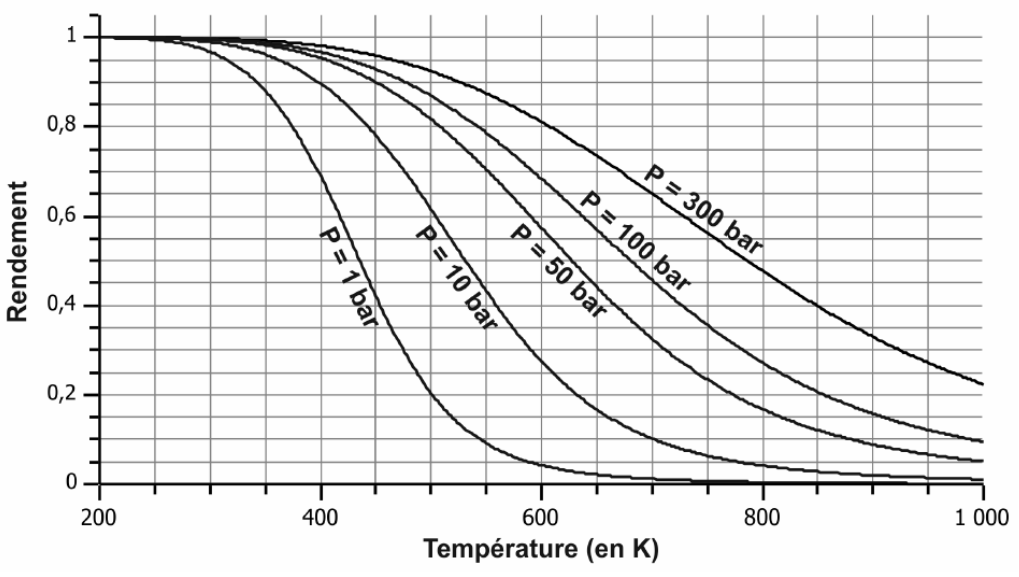
\includegraphics[width=11cm]{pression}}
\end{figure}
On voit que à la température de $700^o K$ à laquelle on va travailler, on à intérêt à travailler à haute pression si on veut optimiser le rendement, dans la mesure du possible bien sûr (travailler à haute pression nécessite beaucoup d'ingénierie et donc d'argent).

\subsubsection{Proportion initiales des réactifs}
Cette fois on cherche comment optimiser $x_{NH_3}$, ce qui revient à jouer sur le quotient réactionnel. On a, les pressions partielles étant définies comme $p_i = x_iP_{tot}$, 
\begin{eqnarray}
K^o = \frac{x_{NH_3}^2}{x_{N_2}x_{H_2}^3}\frac{P_o^2}{P_{tot}^2}
\end{eqnarray}
d'où on déduit 
\begin{eqnarray}
d\ln K^o = d\left(2\ln _{NH_3} - \ln x_{N_2} - 3 \ln x_{H_2} + 2\ln \frac{P_o}{P_{tot}}\right)
\end{eqnarray}
or on se place ici à T et P constantes, et à $x_{NH_3}$ maximal, d'où
\begin{eqnarray}
\frac{dx_{N_2}}{x_{N_2}}  + 3\frac{dx_{H_2}}{x_{H_2}} = 0.
\end{eqnarray}
En utilisant que 
\begin{eqnarray}
x_{NH_3} + x_{N_2} + x_{H_2} =1 \;\mathrm{on\;obtient} \;d x_{N_2} = -dx_{H_2}
\end{eqnarray}
d'où 
\begin{eqnarray}
3x_{N_2} = x_{H_2}
\end{eqnarray}
et ce à chaque instant, notamment au niveau des concentrations initiales $\Rightarrow$ on doit introduire les réactifs dans les proportions stoechiométriques.

\section{Conclusion}
On a pu voir les diverses aspects de l'optimisation d'une réaction chimique, bien que dans la pratique il reste, au niveau industriel, à concevoir les matériels et protocoles permettant de mettre en œuvre les différents points exposés ici.

\section{Plan rectifié :}
enlever loi d'action de masse,\\ 

enlever partie cinétique,\\
 
faire l'application du principe de modération pour l'estérification (on explicite $\mathcal{Q}$, et on montre l'impacte de l'élimination de l'ester dessus).\\

Ne pas parler de physique, on fait un cours de prépa : il leur faut du concret.\\

Il faut expliciter complètement le protocole de la manip introductive\\

Il faut être sû de traiter complètement la dernière partie.

\end{document}